\documentclass[aspectratio=43]{beamer}
\usepackage{tikz}
\usetikzlibrary{arrows.meta, positioning, calc, shapes.geometric}

\tikzset{
    circ/.style = {circle, draw, inner sep=0.5pt, minimum size=10pt, font=\tiny, fill=white},
    exc/.style = {->, thick, >={Stealth[length=2mm, width=1.5mm]}},
    inh/.style = {-{Bar[width=2mm, length=1mm]}, thick}
}

\begin{document}
\begin{frame}{Cortico-Cerebellar Microcircuit}

\vspace{-2mm}
\begin{center}
\resizebox{0.75\textwidth}{!}{%
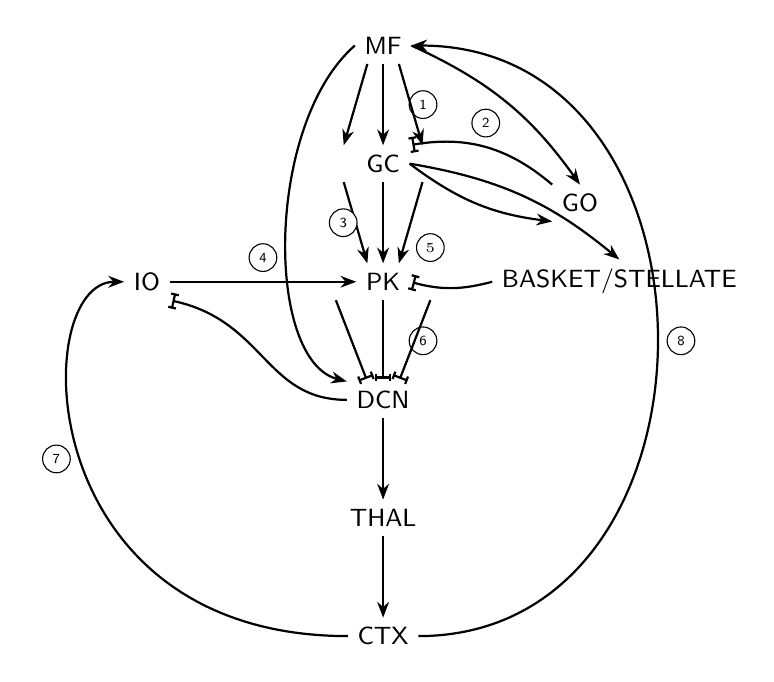
\begin{tikzpicture}[every node/.style={font=\small\sffamily}]
% Central column
\node (MF) at (0, 6.5) {MF};
\node (GC) at (0, 5) {GC};
\node (PK) at (0, 3.5) {PK};
\node (DCN) at (0, 2) {DCN};
\node (THAL) at (0, 0.5) {THAL};
\node (CTX) at (0, -1) {CTX};

% Left side
\node (IO) at (-3, 3.5) {IO};

% Right side
\node (GO) at (2.5, 4.5) {GO};
\node (BS) at (3, 3.5) {BASKET/STELLATE};

% MF -> GC (3 arrows - Diverging)
\draw[exc] ([xshift=-2mm]MF.south) -- ([xshift=-5mm]GC.north);
\draw[exc] (MF.south) -- (GC.north) node[midway, right, xshift=2mm] {\tikz\node[circ]{1};};
\draw[exc] ([xshift=2mm]MF.south) -- ([xshift=5mm]GC.north);

% GC -> PK (3 arrows - Converging)
\draw[exc] ([xshift=-5mm]GC.south) -- ([xshift=-2mm]PK.north);
\draw[exc] (GC.south) -- (PK.north) node[midway, left, xshift=-2mm] {\tikz\node[circ]{3};};
\draw[exc] ([xshift=5mm]GC.south) -- ([xshift=2mm]PK.north);
\node[circ] (circ5) at ([xshift=6mm, yshift=2mm]PK.north) {5}; 

% PK -> DCN (3 inhibitory arrows - Converging)
\draw[inh] ([xshift=-6mm]PK.south) -- ([xshift=-2mm]DCN.north);
\draw[inh] (PK.south) -- (DCN.north) node[midway, right, xshift=2mm] {\tikz\node[circ]{6};};
\draw[inh] ([xshift=6mm]PK.south) -- ([xshift=2mm]DCN.north);

% MF -> GO
\draw[exc, bend left=15] (MF.east) to (GO.north);
% GC -> GO
\draw[exc, bend right=15] (GC.east) to (GO.south west);
% GO -| GC
\draw[inh, bend right=25] (GO.north west) to node[midway, above] {\tikz\node[circ]{2};} (GC.north east);

% GC -> Basket
\draw[exc, bend left=15] (GC.east) to (BS.north);
% Basket -| PK
\draw[inh, bend left=15] (BS.west) to (PK.east);

% IO -> PK
\draw[exc] (IO.east) -- (PK.west) node[midway, above] {\tikz\node[circ]{4};};
% DCN -| IO
\draw[inh] (DCN.west) .. controls (-1.5, 2) and (-1.5, 3) .. (IO.south east);

% MF -> DCN
\draw[exc] (MF.west) .. controls (-1.5, 5.5) and (-1.5, 2.5) .. (DCN.north west);

% CTX -> IO
\draw[exc] (CTX.west) .. controls (-4.5, -1) and (-4.5, 3.5) .. node[midway, left] {\tikz\node[circ]{7};} (IO.west);

% CTX -> MF
\draw[exc] (CTX.east) .. controls (4.5, -1) and (4.5, 6.5) .. node[midway, right] {\tikz\node[circ]{8};} (MF.east);

% Feedforward path
\draw[exc] (DCN.south) -- (THAL.north);
\draw[exc] (THAL.south) -- (CTX.north);
\end{tikzpicture}%
}
\end{center}

\vspace{-1mm}
\begin{center}
\tiny
\renewcommand{\arraystretch}{1.5}
\begin{tabular}{@{}p{0.48\textwidth}p{0.48\textwidth}@{}}
\tikz\node[circ, scale=0.8]{1}; Spatio-temporal expansion & \tikz\node[circ, scale=0.8]{5}; Long term depression \textit{(Anti-Hebbian plasticity)} \\
\tikz\node[circ, scale=0.8]{2}; Sparsity regulation & \tikz\node[circ, scale=0.8]{6}; Inhibitory compression \textit{(Authors didn't think of this!)} \\
\tikz\node[circ, scale=0.8]{3}; Eligibility trace \textit{(Buffer state forward)} & \tikz\node[circ, scale=0.8]{7}; Cortical prediction error \\
\tikz\node[circ, scale=0.8]{4}; Teaching signal & \tikz\node[circ, scale=0.8]{8}; Efference copy \\
\end{tabular}
\end{center}

\end{frame}
\end{document}
